\documentclass[12pt,a4paper]{article}
\usepackage{ctex}  % 支持中文
\usepackage{graphicx}  % 图片支持
\usepackage{hyperref}  % 超链接支持
\usepackage{longtable}  % 长表格支持
\usepackage{array}      % 增强表格功能
\usepackage[left=2.5cm,right=2.5cm,top=2.5cm,bottom=2.5cm]{geometry}  % 页面边距设置
\usepackage{booktabs}   % 美化表格
\usepackage{url}        % URL支持
\usepackage{xfp}
\usepackage{amsmath}
\usepackage{amssymb}
\usepackage{geometry}
\geometry{a4paper, margin=1in}
\usepackage{listings}
\usepackage{xcolor}
\usepackage{calc}                        % 让 \linewidth-2\tabcolsep 可计算
\ExplSyntaxOn                            % 开启 LaTeX3 语法
\cs_new:Npn \real #1 {#1}                % 把 \real{0.30} 展开为 0.30
\ExplSyntaxOff
\usepackage{soul}
\usepackage{microtype}


\sloppy


\lstset{
    numbers=left,
    numberstyle=\tiny\color{gray},
    keywordstyle=\color{blue},
    commentstyle=\color{green},
    basicstyle=\ttfamily,
    breaklines=true,
    breakatwhitespace=true,
    tabsize=2,
    showspaces=false,
    showstringspaces=false
}

\geometry{a4paper, margin=1in}




\renewenvironment{quote}{\begin{quotation}}{\end{quotation}}  % 定义quote环境

\begin{document}

\title{Predicting Olympic Success: Medal Counts, First-Time Medalists, and the Impact of Elite Coaching and Event Dynamics}
\author{}
\date{}
\maketitle


% 把原始mypaper.tex的内容放在这里,但需要进行以下修改:
% 1. 删除顶部的% !TeX root = mypaper.tex
% 2. 将\textbf{1. Introduction}改为\section{Introduction}
% 3. 将\textbf{1.1 Background}改为\subsection{Background}
% 4. 替换所有\protect\phantomsection\label{bookmark*}为简单的\label{sec:*}
% 5. 替换所有\hyperref[bookmark*]为\ref{sec:*}
% 6. 修复表格格式,简化嵌套结构
% 7. 调整图片大小,确保不会超出页面

\section*{Abstract}
This study explores the determinants of national Olympic medal
    performance and the emergence of first-time medalist countries using
    comprehensive datasets from all Summer Olympic Games. Leveraging
    multivariate linear regression and weighted modeling techniques, we
    predict gold and total medal counts for each country, incorporating
    uncertainty estimates and evaluating model performance through robust
    validation metrics. Our projections for the 2028 Los Angeles Summer
    Olympics include detailed prediction intervals, identifying countries
    poised for improvement and those likely to experience declines compared
    to the 2024 Games. Additionally, the model accounts for nations that
    have yet to secure Olympic medals, providing probabilistic forecasts on
    the number of countries expected to achieve their first podium finishes
    in 2028, along with associated confidence levels. The relationship
    between the number and types of Olympic events and national medal
    outcomes is examined, highlighting key sports that significantly
    influence medal prospects for various countries and the impact of host
    nation event selections on performance. Furthermore, we investigate the
    "great coach" effect by employing Difference-in-Differences (DID)
    analysis and case studies of renowned coaches who have led multiple
    national teams to Olympic success. This analysis quantifies the
    contribution of exceptional coaching to medal counts and identifies
    strategic investment areas for three selected countries to enhance their
    Olympic performance through elite coaching. The findings offer novel
    insights into the dynamics of Olympic medal distributions and provide
    actionable recommendations for national Olympic committees to optimize
    their strategies in athlete development, event participation, and
    coaching investment

    \newpage
    \tableofcontents
    \newpage

    
    \section{Introduction}
    
    \subsection{Background}
    
    The Olympic Games have evolved dramatically from their ancient
    origins, when participation was limited to Greek-speaking athletes i .
    Today, they stand as the world\textquotesingle s premier international
    sporting event, symbolized by the iconic five interlocking rings
    designed by Baron Pierre de Coubertin, the founder of the modern
    Olympics z . These rings, reprzesenting the five continents, perfectly
    embody the Games\textquotesingle{} inclusive spirit and global reach.
    
    Since their modern revival in 1896, the Olympics have maintained
    a quadrennial schedule, with events spanning no more than 18 days.
    Throughout their modern history, the Games have demonstrated remarkable
    resilience, having been interrupted only during the two World Wars
    (cancelling the 1916, 1940, and 1944 events) and experiencing a single
    postponement in 2020 due to the global pandemic.
    
    Beyond their sporting significance, the Olympics serve as a
    powerful catalyst for urban transformation and economic development in
    host cities ii. This legacy extends far beyond the competition itself,
    often resulting in improved infrastructure, increased tourism, and
    lasting socioeconomic benefits for the host nation iii.
        
    
    The 2024 Paris Olympics will showcase 329 gold medal events
    across 32 sports iv, with each precious medal containing six grams of
    pure gold and weighing 524 grams in total v. As the Games approach,
    global attention has increasingly focused on the medal count
    predictions, with media outlets and sports analysts from various
    countries already speculating about their nations\textquotesingle{}
    potential performance. This phenomenon reflects how Olympic medals have
    become not just symbols of athletic excellence, but also a measure of
    national pride and sporting prowess on the world stage.
    
    \subsection{Restatement of Problems}
    
    The aim of this study is to develop advanced, data-driven
    predictive models to accurately forecast medal standings for the 2028
    Los Angeles Summer Olympic Games. Utilizing historical data on past
    medal counts, host nations, and event distributions, the study seeks to
    address the following critical challenges:
    
    \textbf{1. Medal Count Prediction:}
    
    Construct predictive models for forecasting the number of gold
    medals and overall medal counts for each National Olympic Committee
    (NOC) participating in the 2028 Games. The models will incorporate
    uncertainty estimates and evaluate their predictive accuracy using
    robust performance metrics, such as Mean Squared Error (MSE), Mean
    Absolute Error(MAE), and the coefficient of determination (R²). These metrics
    will ensure rigorous validation of the models\textquotesingle{}
    reliability and precision.
    
    \textbf{2. Medal Ranking Forecasting:}
    
    Based on the predictive outputs, estimate the final medal
    rankings for each country in the 2028 Olympics, including prediction
    intervals to account for uncertainty. Additionally, identify nations
    likely to exhibit notable improvements or declines in their rankings
    relative to their performance in the 2024 Paris Summer Olympics,
    offering a nuanced understanding of potential shifts in global
    competitiveness.
    
    
    \textbf{3. First-Time Medalists Analysis:}
    
    Extend the predictive framework to include countries that have
    yet to win an Olympic medal. Forecast the number of nations likely to
    secure their first-ever medal at the 2028 Games and estimate the
    probabilities associated with these groundbreaking achievements. This
    analysis will provide insights into the broader inclusivity of the
    Olympic movement.
    
    \textbf{4. Event-Specific Dynamics:}
    
    Analyze the relationship between the number and types of Olympic
    events and the medal performance of competing nations. Identify the most
    critical sports that contribute to the success of different countries
    and assess the influence of event selection by the host nation on
    overall medal outcomes. This aspect will shed light on strategic
    prioritization for both host and non-host countries.
    
    
    \textbf{5. Impact of Coaching Transitions (``Coach Effect''):}
    
    Investigate the potential influence of high-profile coaches
    switching national teams on medal performance. Quantify the contribution
    of this ``coach effect'' and recommend specific sports and countries
    where employing elite coaches could substantially enhance medal
    prospects. This analysis will provide actionable guidance for leveraging
    coaching expertise to maximize competitive advantage.
    
    \subsection{Overview of Our Work}
    
    This study develops a robust framework to predict Olympic medal
    counts and identify potential first-time medalist nations for the 2028
    Los Angeles Summer Olympics. Key steps include:
    
    \textbf{Data Cleaning and Integration:} Merged datasets from 2000
    onwards, focusing on medal tables, host country data, event details, and
    athlete performances to ensure reliability and relevance.
    
    \textbf{Feature Engineering:} Counted total gold, silver, bronze, and
    overall medals for each country since 2000.
    
    \textbf{Medal Count Prediction:} Applied multivariate regression for
    consistent participants, weighted models for irregular participants, and
    direct methods for countries with minimal data.
    
    \textbf{First-Time Medalist Prediction:} Used Random Forest models with
    SMOTE to predict probabilities of countries achieving their first
    Olympic medals, with confidence intervals to ensure precision.
    
    \textbf{Impact of Great Coaches:} Conducted Difference-in-Differences
    (DID) analysis to quantify the effect of elite coaching on national
    medal counts, isolating it from other factors.
    
    \subsection{Data Analysis}
    
    An analysis of Olympic excellence across nearly two and a half
    decades reveals fascinating patterns in the distribution of medals among
    leading sporting nations. The dataset, spanning from 2000 to 2024,
    offers a compelling narrative of international athletic achievement and
    national sporting prowess, illuminating the intricate dynamics of global
    sporting competition.
    
    The perennial fascination with Olympic powerhouses draws our
    attention to an elite circle of nations that have consistently dominated
    the medal tables. Through meticulous analysis of historical data, we can
    identify these Olympic titans who have maintained their reign at the
    pinnacle of sporting excellence. These perennial champions, led by the
    United States and followed closely by sporting giants like China and UK,
    have established themselves as the true emperors of the Olympic arena,
    consistently commanding the upper echelons of the medal standings with
    remarkable persistence.
    
    \begin{figure}[htbp]
        \centering
        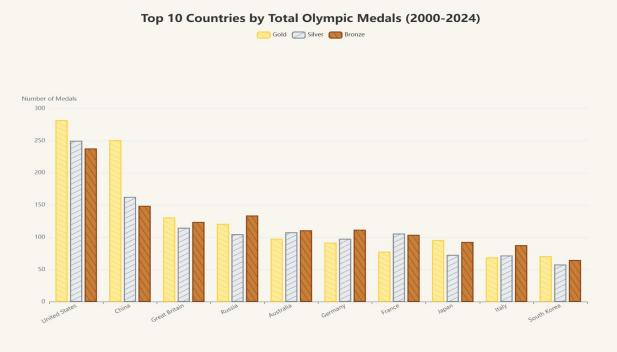
\includegraphics[width=\textwidth]{./media/media/image3.jpeg}
        \caption{\textbf{Top 10 Countries}}
        \label{fig:top10countries}
    \end{figure}
    
    
    A closer examination of the United States\textquotesingle{}
    performance reveals a remarkably balanced medal distribution, with
    consistently high gold medal counts year after year and an impressively
    proportional distribution across gold, silver, and bronze. This stands
    in stark contrast to their closest competitor, China, whose singular
    focus on gold medals reflects a controversial
    
    
    approach to Olympic success. The Chinese strategy, which often
    diminishes the achievements of non-gold medalists, appears to be driven
    by a nationalistic desire to surpass the US gold medal count, feeding
    into a carefully cultivated narrative of national superiority. Yet,
    despite this intense focus on gold medals and the immense pressure
    placed on their athletes, they consistently fall short of overtaking the
    United States\textquotesingle{} overall Olympic dominance.
    
    \begin{figure}[htbp]
        \centering
        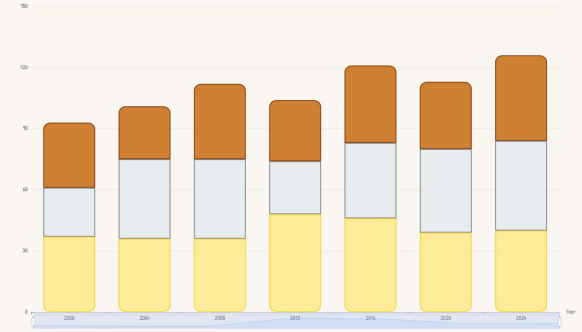
\includegraphics[width=\textwidth]{./media/media/image4.png}
        \caption{\textbf{US Medal Distribution}}
        \label{fig:usmedaldistribution}
    \end{figure}
    
    Within our comprehensive analysis, we\textquotesingle ve
    uncovered a fascinating phenomenon of medal consistency among certain
    nations. While some countries maintain their stable positions through
    sheer sporting supremacy and robust athletic infrastructure, others
    display an intriguing pattern of consistency that defies conventional
    expectations. This remarkable stability in medal acquisition, whether at
    the top tier or in more modest positions, presents an engaging paradox
    in Olympic performance patterns, warranting deeper investigation into
    the underlying factors that contribute to such sustained achievement
    levels.
    \begin{figure}[htbp]
        \centering
        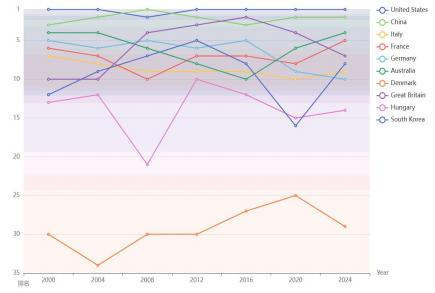
\includegraphics[width=\textwidth]{./media/media/image5.jpeg}
        \caption{\textbf{Olympic Ranking Stability Analysis (2000-2024)}}
        \label{fig:olymprankingstability}
    \end{figure}
    
 
    \section{Model Establishment and Solutions}
    
    \subsection{Forecast 2028 Los Angeles Olympic Games}
    
    \subsubsection{Data Preparation and Cleaning}
    
    We used the data in "summerOly\_athletes.csv" and "" in this
    process, considering the time cycle of the Olympic Games, many athletes
    retired after participating in the two Olympic
    
    
    Games. In addition, the performance level of each country in the
    Olympic Games is related to the comprehensive national strength of the
    country. In addition, the competition system of the pre-2000 Olympic
    Games is also quite different from the present, so we discard all the
    data before 2000 and only intercept the data after 2000 for use.
    
    Because of the different events of each Olympic Games, the
    different events will have a huge impact on the medal. It is very
    important to ensure that the events we predict are present at the 2028
    Olympic Games. We used the latest available 2028 Los Angeles Games
    sports list (available on the official website) as a condition to
    exclude those sports that do not exist at the 2028 Games.
    
    In order to make better use of our time series model, we extend
    it with existing data. We created the historical medal count, starting
    from 2000, adding up gold, silver, bronze, and total medal count as our
    complementary feature. At the same time, to simplify the model, we
    combine the same rows for Sport, and de-duplicate the gold medal
    statistics for team events (because in the athlete table, a team event
    will award a gold medal to each person, but this should only be counted
    once when calculating the national gold medal count).
    
    To categorize events as team-based, we first compiled a list of
    sports inherently involving teams, such as Basketball, Football, and
    Volleyball. Additionally, we identified specific keywords commonly
    associated with team events, including "Team," "Doubles," "Pair,"
    "Mixed," "Four," and "Eight." By examining each event's sport and its
    name, we classified an event as a team event if it belonged to the
    predefined team sports or contained any of the team-related keywords.
    This combined approach ensures a comprehensive and accurate
    identification of team events, facilitating more precise analysis and
    modeling in our study.

    
    As there is no overall information yet on the countries
    participating in the 2028 Olympics, we can only extrapolate using what
    we knowvi. We excluded countries whose last Olympic participation was
    less than 2012. Because these countries are not likely to participate in
    the 2028 Olympic Games, and there is a lack of reference data, we will
    not consider these countries
    
    \begin{quote}
    \protect\phantomsection\label{bookmark28}{}\textbf{3.1.2 Model
    Establishment}
    
    \textbf{For countries that are not absent, we use a multiple linear
    regression model to make predictions.}
    \end{quote}
    
    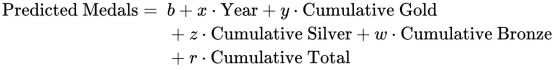
\includegraphics[width=5.76in,height=0.71833in]{./media/media/image6.png}
    
    \begin{longtable}[]{@{}
      >{\raggedright\arraybackslash}p{(\linewidth - 2\tabcolsep) * \real{0.3372}}
      >{\raggedright\arraybackslash}p{(\linewidth - 2\tabcolsep) * \real{0.6628}}@{}}
    \toprule\noalign{}
    \endhead
    \bottomrule\noalign{}
    \endlastfoot
    \begin{minipage}[t]{\linewidth}\raggedright
    \begin{quote}
    \textbf{Variable}
    \end{quote}
    \end{minipage} & \begin{minipage}[t]{\linewidth}\raggedright
    \begin{quote}
    \textbf{Description}
    \end{quote}
    \end{minipage} \\
    \begin{minipage}[t]{\linewidth}\raggedright
    \begin{quote}
    \textbf{Year}
    \end{quote}
    \end{minipage} & \begin{minipage}[t]{\linewidth}\raggedright
    \begin{quote}
    \textbf{The year of the competition}
    \end{quote}
    \end{minipage} \\
    \begin{minipage}[t]{\linewidth}\raggedright
    \begin{quote}
    \textbf{Cumulative Gold}
    \end{quote}
    \end{minipage} & \begin{minipage}[t]{\linewidth}\raggedright
    \begin{quote}
    \textbf{Historical cumulative gold medals}
    \end{quote}
    \end{minipage} \\
    \begin{minipage}[t]{\linewidth}\raggedright
    \begin{quote}
    \textbf{Cumulative Silver}
    \end{quote}
    \end{minipage} & \begin{minipage}[t]{\linewidth}\raggedright
    \begin{quote}
    \textbf{Historical cumulative silver medals}
    \end{quote}
    \end{minipage} \\
    \begin{minipage}[t]{\linewidth}\raggedright
    \begin{quote}
    \textbf{Cumulative Bronze}
    \end{quote}
    \end{minipage} & \begin{minipage}[t]{\linewidth}\raggedright
    \begin{quote}
    \textbf{Historical cumulative bronze medals}
    \end{quote}
    \end{minipage} \\
    \begin{minipage}[t]{\linewidth}\raggedright
    \begin{quote}
    \textbf{Cumulative Total}
    \end{quote}
    \end{minipage} & \begin{minipage}[t]{\linewidth}\raggedright
    \begin{quote}
    \textbf{Historical cumulative total medals}
    \end{quote}
    \end{minipage} \\
    \end{longtable}
    
    \begin{quote}
    \textbf{table 3-1 variable description}
    
    \textbf{For countries that have participated only once or won the same
    number of MEDALS each time, we do not use the model to complicate the
    process, but directly use the number of MEDALS last participated as the
    result of the prediction}
    
    \textbf{For countries with absences in the middle, we use post-2012 data
    to make predictions (if the last participation was taken out before
    2012), and the specific formula is as follows}
    \end{quote}
    
    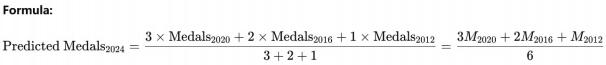
\includegraphics[width=6.29833in,height=0.67in]{./media/media/image7.jpeg}
    
    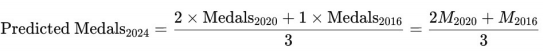
\includegraphics[width=5.64667in,height=0.54in]{./media/media/image8.png}
    
    \begin{quote}
    predicted Medals aoz s=Medals a02o=Ma02o
    
    \textbf{For countries with gaps in participation, the weighted average
    is calculated based on available data, adjusting weights as necessary}
    
    \protect\phantomsection\label{bookmark11-1}{}\textbf{3.1.3 Analysis and
    Evaluation of results}
    
    \textbf{\url{3.1.3.1} Country forecasts are not absent}
    \end{quote}
    
    \textbf{We sampled two representative countries (China and the United
    States) to demonstrate the predictive performance of our model.}
    
    \begin{quote}
    \textbf{The predictive performance of the ARIMA model is evaluated by
    the residual analysis diagram and the comparison between the predicted
    and the actual values.}
    
    \textbf{The residual analysis diagram shows that most of the residual
    errors are concentrated in the range of ±2, indicating that the
    prediction error of the model is small and evenly distributed,
    indicating that the model has a good fitting effect on the whole.}
    
    \textbf{The comparison between the predicted and the actual values
    further verifies the validity of the model. The actual number of MEDALS
    in most sports is highly consistent with the predicted value, reflecting
    the high accuracy of the model in these sports. However, for a small
    number of sports, the deviation may be due to large data fluctuations or
    the model does not adequately capture their specific trends. This
    suggests that in future model optimization, we need to conduct more
    in-depth analysis and adjustment for these underperforming projects.}
    \end{quote}
    
    \textbf{By combining these two charts, we confirm that the ARIMA model
    is stable and reliable in predicting most sports, while identifying
    specific areas that need improvement to improve the overall accuracy of
    the forecast.}
    
    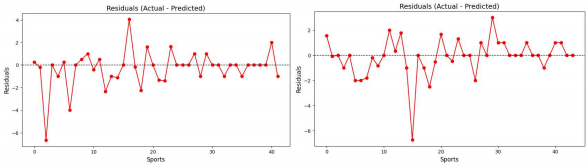
\includegraphics[width=6.115in,height=1.72167in]{./media/media/image9.png}
    
    \begin{quote}
    \textbf{3-1 Residual visualization (left China, right USA)}
    \end{quote}
    
    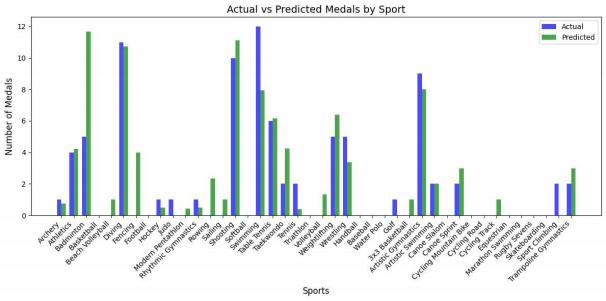
\includegraphics[width=6.29833in,height=3.125in]{./media/media/image10.jpeg}
    
    \begin{quote}
    \textbf{3-2 China Actual vs Predicted Medals Plot}
    \end{quote}
    
    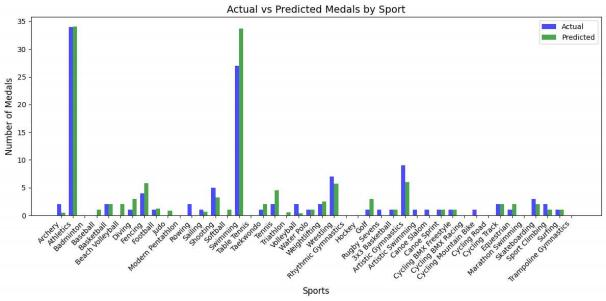
\includegraphics[width=6.29833in,height=3.125in]{./media/media/image11.jpeg}
    
    \begin{quote}
    \textbf{3-3 USA Actual vs Predicted Medals Plot}
    
    \textbf{We also counted the MSE and MAE of the predicted results, as
    shown in the table below}
    
    \textbf{MAE}
    
    \textbf{0.94}
    
    \textbf{table 3-2 MSE \& MAE of China \& USA}
    
    \textbf{\url{3.1.3.2} Projections for countries that have participated
    only once}
    \end{quote}
    
    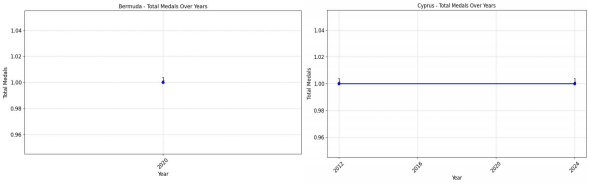
\includegraphics[width=6.12333in,height=1.905in]{./media/media/image12.png}
    
    \begin{quote}
    \textbf{3-4 Bermuda \& Cypurs Total Medals (left-Bermuda, right-Cypurs)}
    
    \textbf{For countries that have only participated in one Olympics or
    that have a fixed number of MEDALS per event, such as Bermuda and
    Cyprus, we keep their MEDALS numbers and do not process or predict them
    too much.}
    
    \textbf{\url{3.1.1.3} For countries absent from participation}
    
    \textbf{We tried some models like Xgboost, ARIMA, but they
    didn\textquotesingle t work well. Analyzing the reasons, we believe that
    the Olympic Games has a very important time factor. Every four years,
    the quality of the contestants changes significantly, and the use of
    overly complex models without the use of external data increases
    entropy. So, for the countries here, we use something like a
    weight-based calculation.}
    
    \textbf{We use Australia as an example here. From the residual analysis
    chart and the actual bar chart, we can see that the prediction ability
    of this method is good for most motions. We also calculated the MSE and
    MAE of the predicted results, which were 1.43 and 0.62, respectively.}
    \end{quote}
    
    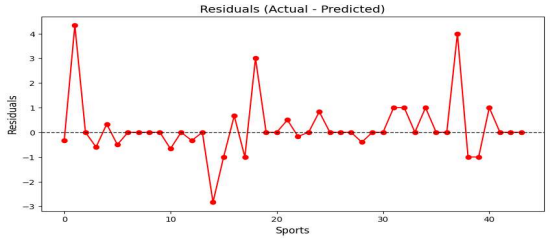
\includegraphics[width=5.71833in,height=2.495in]{./media/media/image13.png}
    
    \begin{quote}
    \textbf{3-5 Australia Residual visualization}
    \end{quote}
    
    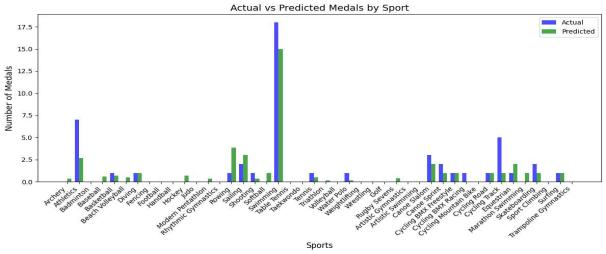
\includegraphics[width=6.30167in,height=2.62667in]{./media/media/image14.jpeg}
    
    \begin{quote}
    \textbf{3-6 Australia Actual vs Predicted Medals Plot}
    
    \textbf{\url{3.1.1.4} Results}
    \end{quote}
    
    \begin{longtable}[]{@{}
      >{\raggedright\arraybackslash}p{(\linewidth - 6\tabcolsep) * \real{0.2501}}
      >{\raggedright\arraybackslash}p{(\linewidth - 6\tabcolsep) * \real{0.2499}}
      >{\raggedright\arraybackslash}p{(\linewidth - 6\tabcolsep) * \real{0.2501}}
      >{\raggedright\arraybackslash}p{(\linewidth - 6\tabcolsep) * \real{0.2498}}@{}}
    \toprule\noalign{}
    \endhead
    \bottomrule\noalign{}
    \endlastfoot
    \begin{minipage}[t]{\linewidth}\raggedright
    \begin{quote}
    \textbf{NOC}
    \end{quote}
    \end{minipage} & \begin{minipage}[t]{\linewidth}\raggedright
    \begin{quote}
    \textbf{Predicted Medal}
    \end{quote}
    \end{minipage} & \begin{minipage}[t]{\linewidth}\raggedright
    \begin{quote}
    \textbf{NOC}
    \end{quote}
    \end{minipage} & \begin{minipage}[t]{\linewidth}\raggedright
    \begin{quote}
    \textbf{Predicted Medal}
    \end{quote}
    \end{minipage} \\
    \begin{minipage}[t]{\linewidth}\raggedright
    \begin{quote}
    \textbf{USA}
    \end{quote}
    \end{minipage} & \begin{minipage}[t]{\linewidth}\raggedright
    \begin{quote}
    \textbf{69}
    \end{quote}
    \end{minipage} & \begin{minipage}[t]{\linewidth}\raggedright
    \begin{quote}
    \textbf{ITA}
    \end{quote}
    \end{minipage} & \begin{minipage}[t]{\linewidth}\raggedright
    \begin{quote}
    \textbf{12}
    \end{quote}
    \end{minipage} \\
    \begin{minipage}[t]{\linewidth}\raggedright
    \begin{quote}
    \textbf{CHN}
    \end{quote}
    \end{minipage} & \begin{minipage}[t]{\linewidth}\raggedright
    \begin{quote}
    \textbf{65}
    \end{quote}
    \end{minipage} & \begin{minipage}[t]{\linewidth}\raggedright
    \begin{quote}
    \textbf{KEN}
    \end{quote}
    \end{minipage} & \begin{minipage}[t]{\linewidth}\raggedright
    \begin{quote}
    \textbf{12}
    \end{quote}
    \end{minipage} \\
    \begin{minipage}[t]{\linewidth}\raggedright
    \begin{quote}
    \textbf{GBR}
    \end{quote}
    \end{minipage} & \begin{minipage}[t]{\linewidth}\raggedright
    \begin{quote}
    \textbf{28}
    \end{quote}
    \end{minipage} & \begin{minipage}[t]{\linewidth}\raggedright
    \begin{quote}
    \textbf{CAN}
    \end{quote}
    \end{minipage} & \begin{minipage}[t]{\linewidth}\raggedright
    \begin{quote}
    \textbf{12}
    \end{quote}
    \end{minipage} \\
    \begin{minipage}[t]{\linewidth}\raggedright
    \begin{quote}
    \textbf{KOR}
    \end{quote}
    \end{minipage} & \begin{minipage}[t]{\linewidth}\raggedright
    \begin{quote}
    \textbf{23}
    \end{quote}
    \end{minipage} & \begin{minipage}[t]{\linewidth}\raggedright
    \begin{quote}
    \textbf{FRA}
    \end{quote}
    \end{minipage} & \begin{minipage}[t]{\linewidth}\raggedright
    \begin{quote}
    \textbf{10}
    \end{quote}
    \end{minipage} \\
    \begin{minipage}[t]{\linewidth}\raggedright
    \begin{quote}
    \textbf{GER}
    \end{quote}
    \end{minipage} & \begin{minipage}[t]{\linewidth}\raggedright
    \begin{quote}
    \textbf{15}
    \end{quote}
    \end{minipage} & \begin{minipage}[t]{\linewidth}\raggedright
    \begin{quote}
    \textbf{UKR}
    \end{quote}
    \end{minipage} & \begin{minipage}[t]{\linewidth}\raggedright
    \begin{quote}
    \textbf{10}
    \end{quote}
    \end{minipage} \\
    \end{longtable}
    
    \begin{quote}
    \textbf{table 3-2 Top10 Priedicted Medal}
    \end{quote}
    
    \begin{longtable}[]{@{}
      >{\raggedright\arraybackslash}p{(\linewidth - 6\tabcolsep) * \real{0.2501}}
      >{\raggedright\arraybackslash}p{(\linewidth - 6\tabcolsep) * \real{0.2499}}
      >{\raggedright\arraybackslash}p{(\linewidth - 6\tabcolsep) * \real{0.2501}}
      >{\raggedright\arraybackslash}p{(\linewidth - 6\tabcolsep) * \real{0.2498}}@{}}
    \toprule\noalign{}
    \endhead
    \bottomrule\noalign{}
    \endlastfoot
    \begin{minipage}[t]{\linewidth}\raggedright
    \begin{quote}
    \textbf{NOC}
    \end{quote}
    \end{minipage} & \begin{minipage}[t]{\linewidth}\raggedright
    \begin{quote}
    \textbf{Predicted Gold}
    \end{quote}
    \end{minipage} & \begin{minipage}[t]{\linewidth}\raggedright
    \begin{quote}
    \textbf{NOC}
    \end{quote}
    \end{minipage} & \begin{minipage}[t]{\linewidth}\raggedright
    \begin{quote}
    \textbf{Pridicted Gold}
    \end{quote}
    \end{minipage} \\
    \begin{minipage}[t]{\linewidth}\raggedright
    \begin{quote}
    \textbf{CHN}
    \end{quote}
    \end{minipage} & \begin{minipage}[t]{\linewidth}\raggedright
    \begin{quote}
    \textbf{43}
    \end{quote}
    \end{minipage} & \begin{minipage}[t]{\linewidth}\raggedright
    \begin{quote}
    \textbf{JAM}
    \end{quote}
    \end{minipage} & \begin{minipage}[t]{\linewidth}\raggedright
    \begin{quote}
    \textbf{8}
    \end{quote}
    \end{minipage} \\
    \begin{minipage}[t]{\linewidth}\raggedright
    \begin{quote}
    \textbf{USA}
    \end{quote}
    \end{minipage} & \begin{minipage}[t]{\linewidth}\raggedright
    \begin{quote}
    \textbf{30}
    \end{quote}
    \end{minipage} & \begin{minipage}[t]{\linewidth}\raggedright
    \begin{quote}
    \textbf{KEN}
    \end{quote}
    \end{minipage} & \begin{minipage}[t]{\linewidth}\raggedright
    \begin{quote}
    \textbf{7}
    \end{quote}
    \end{minipage} \\
    \begin{minipage}[t]{\linewidth}\raggedright
    \begin{quote}
    \textbf{KOR}
    \end{quote}
    \end{minipage} & \begin{minipage}[t]{\linewidth}\raggedright
    \begin{quote}
    \textbf{17}
    \end{quote}
    \end{minipage} & \begin{minipage}[t]{\linewidth}\raggedright
    \begin{quote}
    \textbf{NED}
    \end{quote}
    \end{minipage} & \begin{minipage}[t]{\linewidth}\raggedright
    \begin{quote}
    \textbf{7}
    \end{quote}
    \end{minipage} \\
    \begin{minipage}[t]{\linewidth}\raggedright
    \begin{quote}
    \textbf{GBR}
    \end{quote}
    \end{minipage} & \begin{minipage}[t]{\linewidth}\raggedright
    \begin{quote}
    \textbf{15}
    \end{quote}
    \end{minipage} & \begin{minipage}[t]{\linewidth}\raggedright
    \begin{quote}
    \textbf{CAN}
    \end{quote}
    \end{minipage} & \begin{minipage}[t]{\linewidth}\raggedright
    \begin{quote}
    \textbf{6}
    \end{quote}
    \end{minipage} \\
    \begin{minipage}[t]{\linewidth}\raggedright
    \begin{quote}
    \textbf{GER}
    \end{quote}
    \end{minipage} & \begin{minipage}[t]{\linewidth}\raggedright
    \begin{quote}
    \textbf{11}
    \end{quote}
    \end{minipage} & \begin{minipage}[t]{\linewidth}\raggedright
    \begin{quote}
    \textbf{ITA}
    \end{quote}
    \end{minipage} & \begin{minipage}[t]{\linewidth}\raggedright
    \begin{quote}
    \textbf{6}
    \end{quote}
    \end{minipage} \\
    \end{longtable}
    
    \begin{quote}
    \textbf{table 3-3 Top10 Priedicted Gold}
    \end{quote}
    
    \begin{longtable}[]{@{}
      >{\raggedright\arraybackslash}p{(\linewidth - 6\tabcolsep) * \real{0.2501}}
      >{\raggedright\arraybackslash}p{(\linewidth - 6\tabcolsep) * \real{0.2499}}
      >{\raggedright\arraybackslash}p{(\linewidth - 6\tabcolsep) * \real{0.2501}}
      >{\raggedright\arraybackslash}p{(\linewidth - 6\tabcolsep) * \real{0.2498}}@{}}
    \toprule\noalign{}
    \endhead
    \bottomrule\noalign{}
    \endlastfoot
    \begin{minipage}[t]{\linewidth}\raggedright
    \begin{quote}
    \textbf{NOC}
    \end{quote}
    \end{minipage} & \begin{minipage}[t]{\linewidth}\raggedright
    \begin{quote}
    \textbf{Predicted Silver}
    \end{quote}
    \end{minipage} & \begin{minipage}[t]{\linewidth}\raggedright
    \begin{quote}
    \textbf{NOC}
    \end{quote}
    \end{minipage} & \begin{minipage}[t]{\linewidth}\raggedright
    \begin{quote}
    \textbf{Predicted Silver}
    \end{quote}
    \end{minipage} \\
    \begin{minipage}[t]{\linewidth}\raggedright
    \begin{quote}
    \textbf{USA}
    \end{quote}
    \end{minipage} & \begin{minipage}[t]{\linewidth}\raggedright
    \begin{quote}
    \textbf{39}
    \end{quote}
    \end{minipage} & \begin{minipage}[t]{\linewidth}\raggedright
    \begin{quote}
    \textbf{KOR}
    \end{quote}
    \end{minipage} & \begin{minipage}[t]{\linewidth}\raggedright
    \begin{quote}
    \textbf{7}
    \end{quote}
    \end{minipage} \\
    \begin{minipage}[t]{\linewidth}\raggedright
    \begin{quote}
    \textbf{CHN}
    \end{quote}
    \end{minipage} & \begin{minipage}[t]{\linewidth}\raggedright
    \begin{quote}
    \textbf{22}
    \end{quote}
    \end{minipage} & \begin{minipage}[t]{\linewidth}\raggedright
    \begin{quote}
    \textbf{ITA}
    \end{quote}
    \end{minipage} & \begin{minipage}[t]{\linewidth}\raggedright
    \begin{quote}
    \textbf{6}
    \end{quote}
    \end{minipage} \\
    \begin{minipage}[t]{\linewidth}\raggedright
    \begin{quote}
    \textbf{GBR}
    \end{quote}
    \end{minipage} & \begin{minipage}[t]{\linewidth}\raggedright
    \begin{quote}
    \textbf{13}
    \end{quote}
    \end{minipage} & \begin{minipage}[t]{\linewidth}\raggedright
    \begin{quote}
    \textbf{ESP}
    \end{quote}
    \end{minipage} & \begin{minipage}[t]{\linewidth}\raggedright
    \begin{quote}
    \textbf{6}
    \end{quote}
    \end{minipage} \\
    \end{longtable}
    
    \begin{longtable}[]{@{}
      >{\raggedright\arraybackslash}p{(\linewidth - 2\tabcolsep) * \real{0.4998}}
      >{\raggedright\arraybackslash}p{(\linewidth - 2\tabcolsep) * \real{0.5002}}@{}}
    \toprule\noalign{}
    \endhead
    \bottomrule\noalign{}
    \endlastfoot
    \begin{minipage}[t]{\linewidth}\raggedright
    \begin{quote}
    \textbf{8}
    \end{quote}
    \end{minipage} & \begin{minipage}[t]{\linewidth}\raggedright
    \begin{quote}
    \textbf{CUB}
    \end{quote}
    \end{minipage} \\
    \begin{minipage}[t]{\linewidth}\raggedright
    \begin{quote}
    \textbf{7}
    \end{quote}
    \end{minipage} & \begin{minipage}[t]{\linewidth}\raggedright
    \begin{quote}
    \textbf{CAN}
    \end{quote}
    \end{minipage} \\
    \end{longtable}
    
    \begin{quote}
    \textbf{table 3-4 Top10 Predicted Silver}
    
    \protect\phantomsection\label{bookmark12-1}{}\textbf{3.2 First Olympic
    Medal Prediction Model}
    
    \protect\phantomsection\label{bookmark13-1}{}\textbf{3.2.1 Model
    Development and Feature Engineering}
    
    \textbf{We developed a binary classification model to predict a
    country\textquotesingle s first Olympic medal win in a given year
    (Yes/No), using only internal organizing committee datasets, adhering to
    competition rules.}
    
    \textbf{Data constraints included raw data across tables with format
    inconsistencies and varied country name representations. Standardizing
    country names was crucial for integrating summerOly\_athletes.csv,
    summerOly\_medal\_counts.csv, and summerOly\_hosts.csv.}
    
    \textbf{Key data integration and feature extraction steps included:}
    
    \textbf{NOC Full Name and Abbreviation Unification: Creating a country
    full name to NOC abbreviation mapping from summerOly\_athletes.csv to
    link tables. Country names in the `Team' column were cleaned to ensure
    consistency with NOC codes.}
    
    \textbf{Host Country Information Extraction: Parsing the "City, Country"
    format in summerOly\_hosts.csv `Host' column to extract and link host
    country information. Fuzzy string matching addressed name variations,
    using a similarity threshold (80\%) to match names to the athlete
    dataset\textquotesingle s `Team' column when direct matches failed.}
    
    \textbf{Feature Engineering: Engineered features include:}
    
    \textbf{a. Athlete Participation Features: Total athletes, male/female
    athlete ratio, sport/discipline diversity, athletes per event, Olympics
    participated, years since first participation. These reflect Olympic
    engagement scope.}
    
    \textbf{b. Host Country Features: Host history count, years since last
    hosting, current host status, potentially influencing medal outcomes.}
    
    \textbf{c. Historical Medal Features: Medals from recent Olympics,
    averages over recent Games, and historical totals (under hypothetical
    prior wins -- zero for countries never medaled in training). These
    indicate Olympic strength and trends.}
    
    \protect\phantomsection\label{bookmark31}{}\textbf{3.2.2 Model Training
    and Validation}
    \end{quote}
    
    \textbf{We used a Random Forest Classifier with TimeSeriesSplit
    cross-validation and SMOTE oversampling to manage class imbalance. Model
    performance was evaluated using F1-score, classification report, and
    confusion matrix. Feature importance was analyzed to identify key
    prediction drivers.}
    
    \textbf{On the validation set (2020 \& 2024 data), the model achieved an
    overall accuracy of 0.50. The F1-score for predicting first-time medal
    wins was 0.30, with precision at 0.25 and recall at 0.38 for this class.
    The confusion matrix showed that of 8 actual first-time medal winners, 3
    were correctly identified, and of 20 non-first-time winning countries,
    11 were correctly predicted. Feature importance analysis highlighted
    sport\_diversity\_count, athlete\_count\_total, athlete\_count\_male,
    and event\_entry\_count as most influential, suggesting broader sports
    representation and larger athlete contingents are key indicators. SHAP
    value analysis was technically limited.}
    
    \begin{quote}
    \protect\phantomsection\label{bookmark15-1}{}\textbf{3.2.3 2028 Olympic
    Games First Medal Prediction}
    \end{quote}
    
    \textbf{The model predicted first-time medal probabilities for 77
    countries without prior medals before 2024. Monte Carlo Simulation (5000
    iterations) assessed prediction uncertainty.}
    
    \begin{quote}
    \textbf{Top predicted countries for first medals in 2028 include Guinea,
    Congo (Kinshasa), and Nepal. The Monte Carlo simulation median predicted
    approximately 28 first-time medal-winning countries, with a 95\%
    confidence interval from about 26 to 30.}
    
    \protect\phantomsection\label{bookmark16-1}{}\textbf{3.2.4
    Interpretation and Analysis of Prediction Results}
    
    \textbf{High probabilities for countries like Guinea, Congo (Kinshasa),
    and Nepal may reflect increasing athlete participation, even without
    past medals. Feature importance supports this, linking broader
    participation to first medal likelihood. The Monte Carlo simulation's
    confidence interval (26-30) acknowledges prediction uncertainty.}
    \end{quote}
    
    \textbf{Model limitations include reliance on internal data, potentially
    missing external factors influencing Olympic success. The validation
    F1-score (0.30) indicates limited predictive power for first-time
    winners specifically, with better performance in identifying
    non-first-time winners.}
    
    \begin{quote}
    \textbf{Despite limitations, predictions offer insights for national
    Olympic committees. High-probability countries might benefit from
    continued sports investment. Committees seeking first medals can
    strategically focus on diversifying sports and increasing athlete
    representation, aligning with model-identified key features.}
    
    \protect\phantomsection\label{bookmark17-1}{}\textbf{3.3 Event Selection
    and Hosting Choices}
    \end{quote}
    
    \textbf{Investigating How Event Selection and Hosting Choices Influence
    Medal Outcomes Across Nations in the Olympic Games}
    
    \begin{quote}
    \textbf{This study delves into the profound impact of event selection
    and hosting strategies on medal outcomes, focusing on case studies from
    the United States, Jamaica, and China. By examining trends across
    multiple Olympic Games, the research offers valuable insights into the
    dynamics of national medal success and the strategic decisions shaping
    these outcomes.}
    \end{quote}
    
    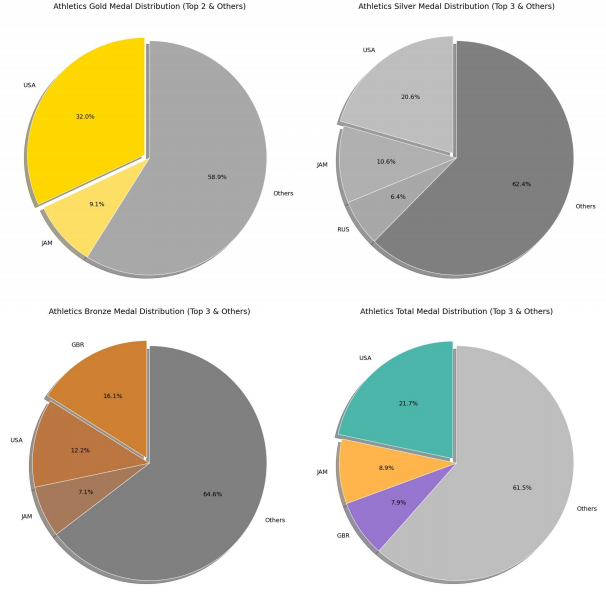
\includegraphics[width=6.29833in,height=6.37833in]{./media/media/image15.png}
    
    \begin{quote}
    \textbf{3-7 Gold, silver, and bronze MEDALS won by the USA in Athletics
    at the 2000-2024 Olympics}
    
    \textbf{An analysis of medal counts in Athletics from the 2000 to 2024
    Olympic Games demonstrates the United States\textquotesingle{} dominance
    in this discipline. Over this period, the U.S. secured 32\% of all gold
    medals in Athletics, significantly outperforming Jamaica, which captured
    9.1\%, placing it in second. Furthermore, the United States accounted
    for 21.7\% of the total medal tally, far exceeding
    Jamaica\textquotesingle s 8.9\%. These figures highlight the strategic
    significance of Athletics in the overall success of Team USA at the
    Olympic Gamesvii (Si,}
    
    \textbf{2018).}
    \end{quote}
    
    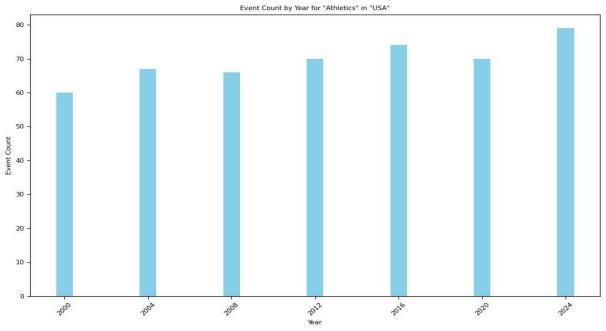
\includegraphics[width=6.30167in,height=3.44333in]{./media/media/image16.jpeg}
    
    \begin{quote}
    \textbf{3-8 The events contained in Athletics at each Olympic Games from
    2000 to 2024}
    \end{quote}
    
    \textbf{The expansion of Athletics as a discipline at the Olympic Games
    is evident from 2000 to 2024, with the number of events increasing from
    60 to nearly 80. This growth reflects heightened global interest and the
    sport\textquotesingle s pivotal role in the Games. The United States has
    benefited considerably from this trend, with its medal count in
    Athletics increasing alongside the number of events, further cementing
    its dominance in the sport. This correlation aligns with previous
    findings that event selection significantly impacts medal success,
    particularly for dominant nations like the U.S.viii (Si, 2018; Katz,
    2024).}
    
    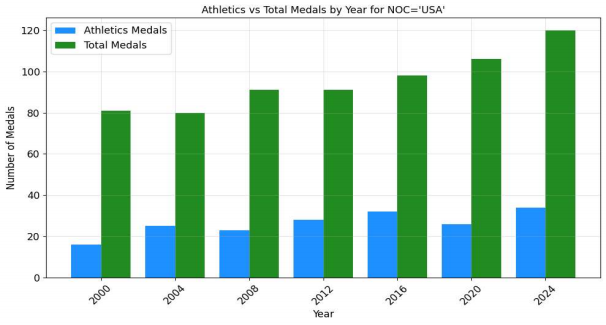
\includegraphics[width=6.30167in,height=3.37333in]{./media/media/image17.png}
    
    \begin{quote}
    \textbf{3-9 The total medals and medals in Athletics of USA from 2000 to
    2024}
    \end{quote}
    
    \textbf{Between 2000 and 2024, the United States\textquotesingle{}
    performance in Athletics saw a remarkable upward trajectory, with gold
    medal counts increasing from 15 to 35 and overall medal counts rising
    from 82 to 120. This trend underscores the vital role of Athletics in
    contributing to the overall success of Team USA. The analysis confirms
    that the increasing emphasis on this discipline has not only enhanced
    medal totals but also bolstered the country\textquotesingle s standing
    in global rankings. Such results resonate with Katz's (2024) argument
    that data-driven predictions and strategic event prioritization are
    integral to optimizing Olympic performance.}
    
    \begin{quote}
    \textbf{Applying a similar analytical lens to other nations,
    Jamaica\textquotesingle s dominance in sprinting events emerges as a
    significant factor in its Olympic success. The nation's medal tally in
    Athletics aligns almost perfectly with its performance in running
    disciplines, highlighting the disproportionate impact of sprint events
    on its overall medal outcomes. This finding is consistent with prior
    research attributing Jamaica\textquotesingle s success to cultural and
    systemic factors that favor sprinting excellence (Taylor, 2015) ix.}
    
    \textbf{In contrast, China's supremacy in Diving reflects a focused
    investment in a single discipline to achieve maximum impact. Diving
    consistently accounts for a substantial proportion of China's gold medal
    tally, showcasing the nation's strategic resource allocation and elite
    coaching systems (Zheng, 2024)x. For instance, Zheng (2024) highlights
    how China's success in Diving stems from both its technical expertise
    and a long-term commitment to nurturing talent in this highly
    specialized field.}
    \end{quote}
    
    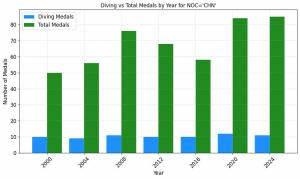
\includegraphics[width=3.115in,height=1.85833in]{./media/media/image18.jpeg}
    
    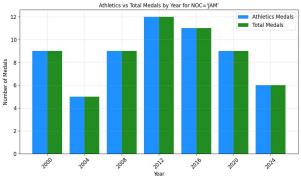
\includegraphics[width=3.12167in,height=1.86167in]{./media/media/image19.jpeg}
    
    \begin{quote}
    \textbf{3-10 The Total medals from JAM \& CHN (left-JAM right-CHN)}
    
    \textbf{3.4 Investigating Factors Influencing Medal Counts: The}
    \protect\phantomsection\label{bookmark18}{}\textbf{"Great Coach Effect"}
    
    \protect\phantomsection\label{bookmark19-1}{}\textbf{3.4.1
    Difference-in-Differences Analysis of Performance Breakthroughs}
    \end{quote}
    
    \textbf{To assess the general impact of performance enhancements
    potentially linked to coaching or program changes, we utilized a
    difference-in-differences (DID) model. This model examines the effect of
    a "treatment" condition, defined by either a significant performance
    breakthrough (exceeding a weighted medal score threshold) or a high
    influx of new athletes, on weighted medal scores.}
    
    \begin{quote}
    \textbf{The DID model specification is:}
    
    weighted\_score=B0+B1X Treat+e
    
    \textbf{where Weighted\_Score represents the weighted medal score, Treat
    is a binary treatment indicator, β0 is the intercept, β 1 is the
    treatment effect coefficient, and ε is the error term. Pooled OLS with
    clustered standard errors was used for estimation.}
    
    \textbf{The results of the DID model reveal a statistically significant
    and positive coefficient for the Treat variable (β 1 = 0.7904, p
    \textless{} 0.0001). This suggests a positive association between the
    defined "treatment" conditions and increased weighted medal scores.
    Figure 1 visualizes the trend comparison between treated and control
    groups, while Figure 2 presents the coefficient estimates.}
    \end{quote}
    
    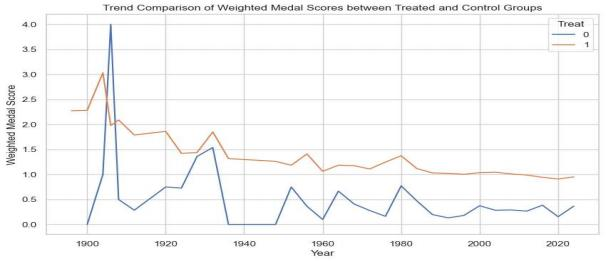
\includegraphics[width=6.30167in,height=2.71333in]{./media/media/image20.jpeg}
    
    \begin{quote}
    \textbf{3-11 Trend Comparison of Weighted Medal Scores between Treated
    and Control Groups .}
    
    \textbf{The blue line represents the average weighted medal score trend
    for the control group (Treat=0), while the orange line represents the
    trend for the treated group (Treat=1).}
    \end{quote}
    
    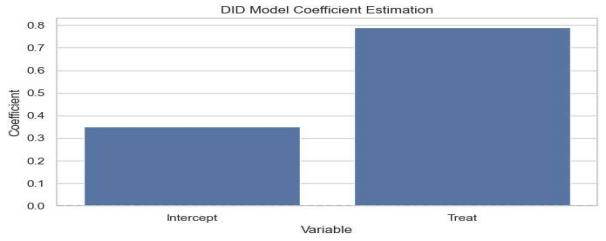
\includegraphics[width=6.30167in,height=2.49667in]{./media/media/image21.jpeg}
    
    \begin{quote}
    \textbf{3-12 DID Model Coefficient Estimation.}
    
    \textbf{This bar chart displays the estimated coefficients for the
    Intercept and Treat variables from the DID model. Error bars (if
    applicable) would represent confidence intervals for the coefficient
    estimates.}
    
    \textbf{The positive and significant coefficient in the DID model
    suggests that factors captured by our "treatment" definition,
    potentially including effective coaching interventions, are associated
    with improved medal performance. However, to explore the "great coach
    effect" more directly, we now turn to case studies of specific renowned
    coaches.}
    
    \protect\phantomsection\label{bookmark20-1}{}\textbf{3.4.2 Case Study
    Evidence: Lang Ping, Béla Károlyi, and Bob Bowman}
    
    \textbf{To delve deeper into the potential "great coach effect," we
    conducted case studies focusing on three prominent coaches: Lang Ping
    (Volleyball), Béla Károlyi (Gymnastics), and Bob Bowman (Swimming).
    These coaches are widely recognized for their exceptional achievements
    and influence within their respective sports.}
    
    \textbf{Lang Ping and Chinese Women\textquotesingle s Volleyball}
    \end{quote}
    
    \textbf{The analysis of Lang Ping\textquotesingle s coaching tenures
    with the Chinese women\textquotesingle s volleyball team reveals a
    compelling positive impact. As shown in 3-13, weighted medal scores and
    performance breakthrough probabilities were significantly higher during
    her coaching periods compared to non-coaching periods.}
    
    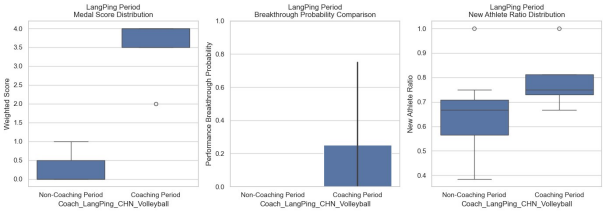
\includegraphics[width=6.29833in,height=2.20167in]{./media/media/image22.png}
    
    \begin{quote}
    \textbf{3-13: Lang Ping Coaching Period Impact on Chinese
    Women\textquotesingle s Volleyball.}
    
    \textbf{(a) Box plot comparing weighted medal score distributions.}
    
    \textbf{(b) Bar chart comparing performance breakthrough probabilities.}
    
    \textbf{(c) Box plot comparing new athlete ratio distributions.}
    
    \textbf{The data strongly suggests that Lang Ping\textquotesingle s
    coaching expertise contributed significantly to the medal success of the
    Chinese women\textquotesingle s volleyball program, providing strong
    evidence for the "great coach effect" in this specific context.}
    
    \textbf{Béla Károlyi and US Women\textquotesingle s Gymnastics}
    
    \textbf{The case of Béla Károlyi and US women\textquotesingle s
    gymnastics, presented in 3-14, offers a more nuanced perspective. While
    a slight increase in average weighted medal score is observed during his
    coaching-associated years, the performance breakthrough rate is lower.}
    \end{quote}
    
    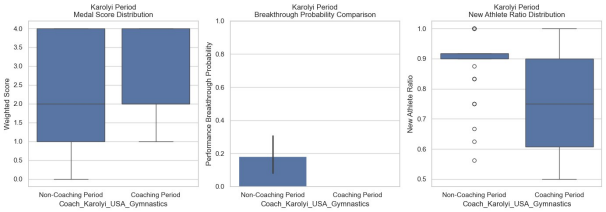
\includegraphics[width=6.29833in,height=2.20167in]{./media/media/image23.png}
    
    \begin{quote}
    \textbf{3-14: Béla Károlyi Coaching Period Impact on US
    Women\textquotesingle s Gymnastics.}
    
    \textbf{(a) Box plot of weighted medal score distributions.}
    
    \textbf{(b) Bar chart of performance breakthrough probabilities.}
    
    \textbf{(c) Box plot of new athlete ratio distributions.}
    
    \textbf{This suggests that Károlyi\textquotesingle s influence may be
    characterized by sustained high performance and athlete development
    rather than solely breakthrough events, indicating a different
    manifestation of potential coaching impact.}
    
    \textbf{Bob Bowman and US Swimming}
    
    \textbf{3-15 presents the analysis for Bob Bowman and US swimming.
    Contrary to expectations,}
    
    \textbf{weighted medal scores and breakthrough probabilities are
    slightly lower during his coaching years.}
    \end{quote}
    
    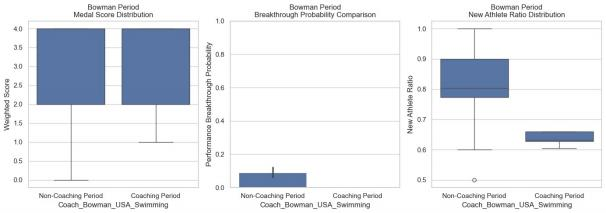
\includegraphics[width=6.29833in,height=2.20167in]{./media/media/image24.jpeg}
    
    \begin{quote}
    \textbf{3-15: Bob Bowman Coaching Period Impact on US Swimming.}
    
    \textbf{(a) Box plot of weighted medal score distributions.}
    
    \textbf{(b) Bar chart of performance breakthrough probabilities.}
    
    \textbf{(c) Box plot of new athlete ratio distributions.}
    
    \textbf{Several factors could explain this:}
    
    \textbf{● Ceiling Effect: US swimming was already a dominant force
    before Bowman\textquotesingle s tenure.}
    
    \textbf{Further significant increases in weighted medal scores might be
    inherently difficult to achieve due to a performance ceiling.}
    
    \textbf{● Focus on Individual Excellence: Bowman\textquotesingle s
    impact might be highly concentrated on individual athletes like Michael
    Phelps. Our analysis, aggregated at the national team level, might not
    fully capture the nuances of his individual athlete development
    expertise.}
    
    \textbf{● Broader Systemic Factors: US swimming\textquotesingle s
    overall success is likely influenced by a complex system of athlete
    development, funding, and infrastructure, beyond the influence of a
    single coach, even one as prominent as Bowman.}
    
    \protect\phantomsection\label{bookmark21-1}{}\textbf{3.4.3 Coach
    Replacement Priority Analysis and Recommendations}
    
    \textbf{To provide actionable recommendations for Olympic committees, we
    conducted a coach replacement priority analysis to identify
    country-sport combinations where investing in a "great coach" might be
    most impactful. This analysis ranks combinations based on a "Priority
    Score" calculated from factors indicating declining performance and
    athlete turnover. The Priority Score is derived from:}
    
    \textbf{● Score\_Trend (Weighted Medal Score Trend): Negative trend
    indicates declining performance, increasing priority.}
    
    \textbf{● New\_Ratio\_mean (Average New Athlete Ratio): Lower new
    athlete ratio (higher athlete retention/staleness) increases priority.}
    
    \textbf{● Score\_MA3\_last (Last 3-year Moving Average of Weighted
    Score): Lower recent performance increases priority.}
    \end{quote}
    
    \begin{longtable}[]{@{}
      >{\raggedright\arraybackslash}p{(\linewidth - 12\tabcolsep) * \real{0.0983}}
      >{\raggedright\arraybackslash}p{(\linewidth - 12\tabcolsep) * \real{0.1019}}
      >{\raggedright\arraybackslash}p{(\linewidth - 12\tabcolsep) * \real{0.1694}}
      >{\raggedright\arraybackslash}p{(\linewidth - 12\tabcolsep) * \real{0.2016}}
      >{\raggedright\arraybackslash}p{(\linewidth - 12\tabcolsep) * \real{0.1428}}
      >{\raggedright\arraybackslash}p{(\linewidth - 12\tabcolsep) * \real{0.1428}}
      >{\raggedright\arraybackslash}p{(\linewidth - 12\tabcolsep) * \real{0.1432}}@{}}
    \toprule\noalign{}
    \endhead
    \bottomrule\noalign{}
    \endlastfoot
    \begin{minipage}[t]{\linewidth}\raggedright
    \begin{quote}
    \textbf{Rank}
    \end{quote}
    \end{minipage} & \begin{minipage}[t]{\linewidth}\raggedright
    \begin{quote}
    \textbf{NOC}
    \end{quote}
    \end{minipage} & \begin{minipage}[t]{\linewidth}\raggedright
    \begin{quote}
    \textbf{Sport}
    \end{quote}
    \end{minipage} & \begin{minipage}[t]{\linewidth}\raggedright
    \begin{quote}
    \textbf{Event}
    \end{quote}
    \end{minipage} & \begin{minipage}[t]{\linewidth}\raggedright
    \begin{quote}
    \textbf{Priority Score}
    \end{quote}
    \end{minipage} & \begin{minipage}[t]{\linewidth}\raggedright
    \begin{quote}
    \textbf{Score Trend}
    \end{quote}
    \end{minipage} & \begin{minipage}[t]{\linewidth}\raggedright
    \begin{quote}
    \textbf{New Ratio mean}
    \end{quote}
    \end{minipage} \\
    \begin{minipage}[t]{\linewidth}\raggedright
    \begin{quote}
    \textbf{1}
    \end{quote}
    \end{minipage} & \begin{minipage}[t]{\linewidth}\raggedright
    \begin{quote}
    \textbf{SLO}
    \end{quote}
    \end{minipage} & \begin{minipage}[t]{\linewidth}\raggedright
    \begin{quote}
    \textbf{Rowing}
    \end{quote}
    \end{minipage} & \begin{minipage}[t]{\linewidth}\raggedright
    \begin{quote}
    \textbf{Rowing Men\textquotesingle s Double Sculls}
    \end{quote}
    \end{minipage} & \begin{minipage}[t]{\linewidth}\raggedright
    \begin{quote}
    \textbf{0.724}
    \end{quote}
    \end{minipage} & \begin{minipage}[t]{\linewidth}\raggedright
    \begin{quote}
    \textbf{0.75}
    \end{quote}
    \end{minipage} & \begin{minipage}[t]{\linewidth}\raggedright
    \begin{quote}
    \textbf{0.685}
    \end{quote}
    \end{minipage} \\
    \begin{minipage}[t]{\linewidth}\raggedright
    \begin{quote}
    \textbf{2}
    \end{quote}
    \end{minipage} & \begin{minipage}[t]{\linewidth}\raggedright
    \begin{quote}
    \textbf{ITA}
    \end{quote}
    \end{minipage} & \begin{minipage}[t]{\linewidth}\raggedright
    \begin{quote}
    \textbf{Modern Pentathlon}
    \end{quote}
    \end{minipage} & \begin{minipage}[t]{\linewidth}\raggedright
    \begin{quote}
    \textbf{Modern}
    
    \textbf{Pentathlon Men\textquotesingle s Team}
    \end{quote}
    \end{minipage} & \begin{minipage}[t]{\linewidth}\raggedright
    \begin{quote}
    \textbf{0.672}
    \end{quote}
    \end{minipage} & \begin{minipage}[t]{\linewidth}\raggedright
    \begin{quote}
    \textbf{0.75}
    \end{quote}
    \end{minipage} & \begin{minipage}[t]{\linewidth}\raggedright
    \begin{quote}
    \textbf{0.556}
    \end{quote}
    \end{minipage} \\
    \begin{minipage}[t]{\linewidth}\raggedright
    \begin{quote}
    \textbf{3}
    \end{quote}
    \end{minipage} & \begin{minipage}[t]{\linewidth}\raggedright
    \begin{quote}
    \textbf{BRA}
    \end{quote}
    \end{minipage} & \begin{minipage}[t]{\linewidth}\raggedright
    \begin{quote}
    \textbf{Sailing}
    \end{quote}
    \end{minipage} & \begin{minipage}[t]{\linewidth}\raggedright
    \begin{quote}
    \textbf{Sailing Men\textquotesingle s}
    
    \textbf{Two Person}
    
    \textbf{Keelboat}
    \end{quote}
    \end{minipage} & \begin{minipage}[t]{\linewidth}\raggedright
    \begin{quote}
    \textbf{0.671}
    \end{quote}
    \end{minipage} & \begin{minipage}[t]{\linewidth}\raggedright
    \begin{quote}
    \textbf{0.75}
    \end{quote}
    \end{minipage} & \begin{minipage}[t]{\linewidth}\raggedright
    \begin{quote}
    \textbf{0.552}
    \end{quote}
    \end{minipage} \\
    \end{longtable}
    
    \begin{quote}
    \textbf{table 3-1 Top 3 Country-Sport-Event Combinations for Coach
    Replacement}
    
    \textbf{3-15,16,17 further illustrate the recent performance trends for
    these top three combinations, showing the decline in Weighted\_Score and
    New\_Ratio over the past three Olympic cycles.}
    \end{quote}
    
    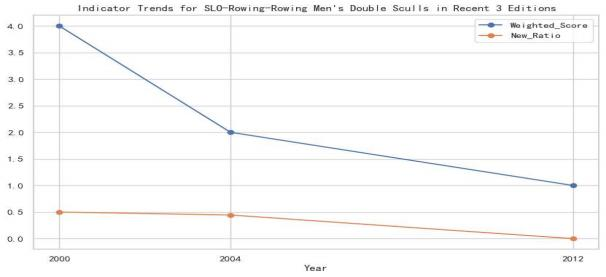
\includegraphics[width=6.30167in,height=2.86667in]{./media/media/image25.jpeg}
    
    \begin{quote}
    \textbf{3-16: Recent Performance Trends for BRA-Sailing-Sailing
    Men\textquotesingle s Two Person Keelboat. Line chart showing
    Weighted\_Score and New\_Ratio trends over the last three Olympic
    cycles.}
    \end{quote}
    
    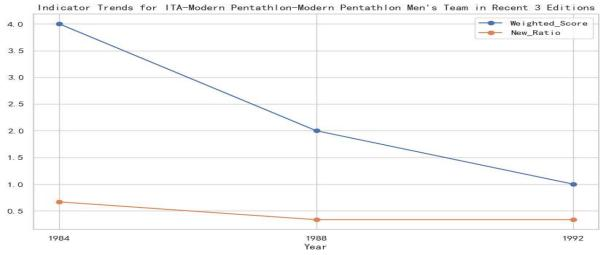
\includegraphics[width=6.30167in,height=2.64833in]{./media/media/image26.jpeg}
    
    \begin{quote}
    \textbf{3-17: Recent Performance Trends for SLO-Rowing-Rowing
    Men\textquotesingle s Double Sculls. Line chart showing Weighted\_Score
    and New\_Ratio trends over the last three Olympic cycles.}
    \end{quote}
    
    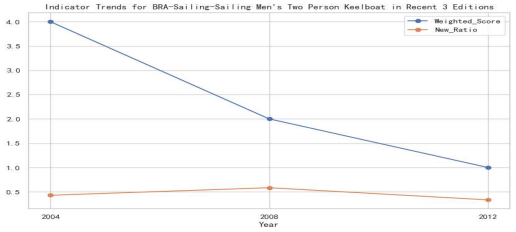
\includegraphics[width=5.36333in,height=2.40666in]{./media/media/image27.png}
    
    \begin{quote}
    \textbf{3-18: Recent Performance Trends for ITA-Modern Pentathlon-Modern
    Pentathlon Men\textquotesingle s}
    
    \textbf{Team. Line chart showing Weighted\_Score and New\_Ratio trends
    over the last three Olympic}
    
    \textbf{cycles.}
    
    \textbf{Based on this analysis, we recommend that the Olympic committees
    of Slovenia (SLO), Italy (ITA), and Brazil (BRA) should consider
    investing in "great coaches" for Rowing Men\textquotesingle s Double
    Sculls, Modern Pentathlon Men\textquotesingle s Team, and Sailing
    Men\textquotesingle s Two Person Keelboat, respectively. These
    combinations exhibit declining performance trends and potentially
    indicate a need for strategic coaching intervention to revitalize their
    medal prospects. Estimating the precise impact is challenging, but based
    on the positive effects observed in the Lang Ping case and the average
    treatment effect from the DID model, strategic investment in a "great
    coach" could potentially reverse the declining performance trend and
    lead to a noticeable improvement in weighted medal scores for these
    specific combinations in future Olympics. Such investment should be
    considered a priority to maximize medal potential in these sports.}
    
    \protect\phantomsection\label{bookmark22-1}{}\textbf{4 Conclusion}
    \end{quote}
    
    \textbf{This study provides a comprehensive analysis of Olympic
    athletics data, revealing key patterns in medal distribution. Gold
    medals show a high concentration among a few nations, reflecting their
    advantages in training, resources, and athlete development. In contrast,
    silver and bronze medals are more broadly distributed, showcasing the
    competitive presence of more nations. Total medal counts highlight
    cumulative impacts, offering a holistic view of national athletic
    strength.}
    
    \begin{quote}
    \textbf{Key Insights for Olympic Strategies}
    
    \textbf{Resource Optimization: Invest in high-potential disciplines and
    athlete development to maximize gold and overall medal counts.}
    
    \textbf{Diversified Development: Engage in multiple athletics events to
    reduce reliance on single disciplines and achieve balanced growth.}
    
    \textbf{Infrastructure and Training: Strengthen facilities, improve
    training environments, and focus on systematic athlete development,
    including psychological resilience.}
    
    \textbf{Broader Factors Influencing Success}
    
    \textbf{Olympic success is shaped by socioeconomic factors (economic
    power, population, societal development), cultural and policy support
    (sports culture, government backing), and technology and innovation
    (advanced training, scientific nutrition, and cutting-edge methods).}
    
    \textbf{Future Research Directions}
    
    \textbf{Performance Metrics: Incorporate detailed athlete data
    (training, injuries, competition) to improve predictive models.}
    
    \textbf{Socioeconomic Analysis: Study the impact of economic and social
    factors on Olympic outcomes.}
    
    \textbf{Interdisciplinary Research: Integrate sports science, sociology,
    and economics to build comprehensive models.}
    
    \textbf{Dynamic Data Analysis: Use time-series models to track and
    improve national Olympic strategies.}
    
    \textbf{These insights aim to support nations in crafting data-driven
    and effective strategies, contributing to global sports development.}
    
    \protect\phantomsection\label{bookmark23-1}{}\textbf{5 Reference}
    
    \textbf{i}
    
    \textbf{ii iii}
    \end{quote}
    
    \textbf{Swaddling J (2000) The ancient Olympic games. Austin, TX:
    University of Texas Press Waitt G (2003) Social impacts of the Sydney
    Olympics. Ann Tourism Res 30: 194--215.}
    
    \begin{quote}
    \textbf{Ben-Naim E, Vazquez F, Redner S (2005) What is the most
    competitive sport? J Korean Phys Soc 50: 124.}
    
    \textbf{iv Paris 2024 unveils Paralympic and Olympic Games medals.
    International Paralympic Committee. {[}2024-08-02{]}. (\ul{link})}
    
    \textbf{v Paris 2024 unveils Paralympic and Olympic Games medals.
    International Paralympic Committee. {[}2024-08-02{]}. (\ul{link})}
    
    \textbf{vi Singh, P., Sharma, A., \& Verma, K. (2024). Predicting Medal
    Counts in Olympics Using Machine Learning Algorithms: A Comparative
    Analysis. ResearchGate.}
    
    \textbf{vii Si, J. (2018). Olympic Game Medal Count Analysis.
    ScholarWorks.}
    
    \textbf{viii Katz, M. (2024). A Data-Driven Approach to Medal Counts
    Reimagines Olympic Ranking System. Yeshiva University News.}
    
    \textbf{ix Taylor, O. W. (2015). It\textquotesingle s Culture, Not
    Genes: Explaining Why Jamaican Sprinters Dominate. JSTOR.}
    
    \textbf{x Zheng, J. (2024). Exploring China\textquotesingle s Success at
    the Olympic Games: A Competitive Advantage Approach. ResearchGate.}
    
    \textbf{AI Use Report:}
    
    \textbf{Formal Declaration of Non-Utilization of Artificial
    Intelligence}
    
    \textbf{Declaration of Authenticity}
    
    \textbf{We, hereby, formally and unequivocally declare that no
    Artificial Intelligence (AI) tools, platforms, or systems were employed
    at any stage in the creation, preparation, or completion of this
    document. All content herein, including but not limited to analysis,
    composition, data interpretation, and conclusions, is solely the result
    of independent human effort, critical thinking, and intellectual
    diligence.}
    
    \textbf{Assurance of Non-AI Involvement}
    
    \textbf{This document represents a product of entirely manual processes,
    crafted with meticulous attention to detail and without any reliance on
    AI-generated content or assistance. No AI models, algorithms, or related
    technologies were utilized to generate, draft, or review any portion of
    this work.}
    
    \textbf{Adherence to Ethical Standards}
    
    \textbf{In alignment with the highest standards of integrity and
    professional ethics, this declaration affirms my unwavering commitment
    to producing original and authentic work. The methodologies, arguments,
    and conclusions contained herein are exclusively derived from human
    expertise and effort.}
    
    \textbf{Verification and Transparency}
    
    \textbf{To further reinforce this declaration, I remain fully prepared
    to provide any necessary evidence, documentation, or clarification
    regarding the processes followed in the development of this document.
    This includes demonstrating that all work was completed without the
    influence or intervention of any AI technologies.}
    \end{quote}
    



% 内容继续...

\end{document}